\documentclass[prb,twocolumn,superscriptaddress,amsmath,amssymb,floatfix]{revtex4-2}
\usepackage{graphicx}
\usepackage{bm}
\usepackage{dcolumn}
\usepackage[colorlinks=true,linkcolor=blue,citecolor=blue,urlcolor=blue]{hyperref}

\setcounter{topnumber}{3}\setcounter{bottomnumber}{2}\setcounter{totalnumber}{5}\setcounter{dbltopnumber}{2}
\renewcommand{\topfraction}{0.92}\renewcommand{\bottomfraction}{0.6}\renewcommand{\textfraction}{0.08}
\renewcommand{\floatpagefraction}{0.75}\renewcommand{\dbltopfraction}{0.92}\renewcommand{\dblfloatpagefraction}{0.75}
\newcommand{\Md}{M_{\rm dice}}
\newcommand{\eps}{\varepsilon}

\begin{document}

\title{Quantum order by disorder among lozenge tilings:\\
a staircase of hub-free crystals between the Lieb ferrimagnet and the antiferromagnet}

\author{Changyeon Won}
\email{cywon@khu.ac.kr}
\affiliation{Department of Physics, Kyung Hee University, Seoul 02447, Republic of Korea}

\date{\today}

\begin{abstract}
Lozenge tilings of the triangular lattice form an extensive family of bipartite networks that interpolates between the dice lattice, a Lieb ferrimagnet with the largest possible sublattice imbalance, and square-type tilings, which are compensated antiferromagnets. For the classical Heisenberg antiferromagnet all of these networks have exactly the same ground-state energy. We show that quantum fluctuations lift this degeneracy through a simple and local mechanism. To leading order the zero-point energy is a sum of single-site terms $\eps(z)$ that depend only on the coordination $z$ (residual $\approx2\times10^{-4}J$ per site in and out of sample), and $\eps(z)$ is convex. Because every lozenge tiling has the same mean coordination $\langle z\rangle=4$, Jensen's inequality selects the uniform square-type tiling, with a selection energy that scales as $JS$. A magnetic field favors the dice tiling through its Lieb moment and competes with this selection. Sign-free quantum Monte Carlo simulations for spins $S=\frac12$ to $\frac32$, combined with an exhaustive enumeration of periodic tilings with up to 36 sites per cell, show that, within the searched space, this competition does not produce a single jump. It instead produces a staircase of periodic crystals with magnetization $\Md/6$, $\Md/3$, $\Md/2$ and $2\Md/3$, each stable over $0.03$--$0.06J$ for $S=\frac12$. The deepest crystal, at $\Md/2$ ($0.168J<h<0.212J$), contains no sixfold hubs at all. Its coordinations are $z=3,4,5$ in equal proportions. We show that sublattice imbalance is carried most cheaply by pairs of $z=3$ and $z=5$ sites, so the $\Md/2$ crystal, the densest hub-free tiling we find, marks a kink of the leading-order energy. This makes the $\Md/2$ and $2\Md/3$ plateaus robust, whereas the low-field plateaus rest on smaller, arrangement-dependent energies. Domain walls between dice and square regions carry negative energy, so mixed structures beat phase separation; all irregular networks we generated lie above the crystals. The step fields are independent of $S$ in units of $J$. In an effective model of tiling fluctuations the $\Md/2$ crystal melts at $T\simeq0.02$--$0.03J$, and local-flip dynamics become kinetically trapped on cooling. Lifting each tiling to its stepped surface in $\mathbb Z^3$ makes $z$ an exact measure of discrete Gaussian curvature and the Lieb moment an exact sublattice-staggered total curvature. In this language zero field selects folded, curvature-free surfaces, and the field crumples them with conical defects. We give the spin-deviation, entanglement, and dynamical-structure-factor signatures of each crystal, and discuss realizations in $\pi$-magnetic nanographenes, atom-by-atom spin arrays, and programmable quantum simulators.
\end{abstract}

\maketitle

\begin{figure*}[t]
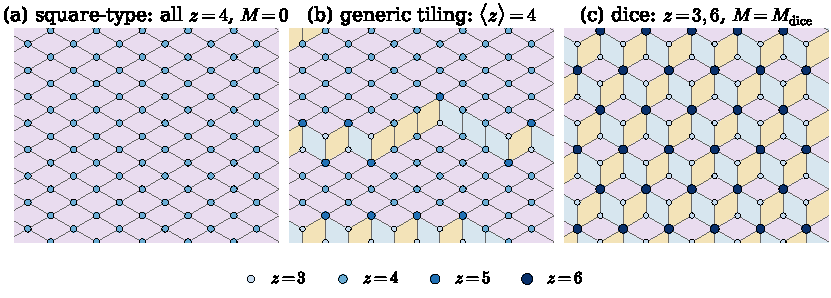
\includegraphics[width=\textwidth]{figs/fig1_tilings.pdf}
\caption{Lozenge tilings of the triangular lattice and the bipartite networks they define. Rhombi are shaded by orientation, and sites are colored and sized by coordination $z$. (a)~Square-type tiling: all $z=4$, compensated ($M=0$). (b)~A generic tiling, with $z$ varying from site to site; every tiling has $\langle z\rangle=4$. (c)~Dice lattice: sixfold hubs and threefold rims, Lieb moment $\Md=SN/3$. All tilings have the same classical energy $-2JS^2N$.}
\label{fig:tilings}
\end{figure*}

%=====================================================================
\section{Introduction}
%=====================================================================

Order by disorder is the selection of a subset of classically degenerate ground states by fluctuations~\cite{Villain1980,Henley1989}. In frustrated magnets the degenerate manifold is usually a family of spin configurations on a \emph{fixed} lattice. Thermal or quantum fluctuations then pick the configurations with the softest excitation spectrum, most often collinear or coplanar ones. In this paper we study a different kind of degeneracy, one in which the object that is degenerate is the \emph{lattice itself}.

Consider the lozenge (rhombus) tilings of the triangular lattice. Each tiling is obtained by pairing every up triangle with one of its down neighbors into a rhombus and deleting the shared edge. The remaining bonds form a planar bipartite graph in which every site has coordination $3\le z\le6$ and the mean coordination is exactly $\langle z\rangle=4$ [Fig.~\ref{fig:tilings}]. Two extreme members of this family are familiar. The dice ($\mathcal{T}_3$) lattice~\cite{Sutherland1986,Vidal1998} has sixfold hubs and threefold rims. The square-type tiling has only fourfold sites and is topologically the square lattice. By Lieb's theorem~\cite{Lieb1989}, the Heisenberg antiferromagnet on any of these graphs has a ground state with total spin $S_{\rm tot}=S|N_A-N_B|$. The dice lattice is therefore a ferrimagnet with the largest possible moment $\Md=SN/3$, while the square-type tiling is compensated. The family thus spans ferrimagnets and antiferromagnets continuously.

For classical spins every tiling has the same energy, $E_{\rm cl}=-JS^2N_b=-2JS^2N$, because every tiling has $N_b=2N$ bonds and collinear N\'eel order satisfies all of them. The number of tilings grows exponentially with $N$. Quantum mechanically the degeneracy is lifted, and two natural questions follow. Which lattice do quantum fluctuations select, and why? And how does a magnetic field, which couples directly to the Lieb moment and therefore favors the dice tiling, compete with that selection?

Quantum spins on dice-derived networks have been studied by Jagannathan, Wessel and co-workers~\cite{Jagannathan2006,Szallas2009,Jagannathan2012,Jagannathan2013}. They found that local ``phason flips'' of a staggered dice lattice raise the quantum ground-state energy and enhance the staggered moment~\cite{Jagannathan2012}, and that domain walls between phason domains carry a positive line energy ($\approx0.062J/a$) and feel a Casimir-like $1/d$ interaction~\cite{Jagannathan2013}. Their reference structure, the staggered dice lattice (SDL), is itself a lozenge tiling with coordinations $z=3,4,5$ in equal numbers and $N_A=N_B$. Those works kept the two sublattices balanced ($N_A=N_B$), considered random or dilute flips, and did not include a field. The questions posed above involve sectors with different sublattice imbalance, systematic control of that imbalance, and the competition with a Zeeman field. To our knowledge they have not been addressed.

Our main results are as follows.
(i) The zero-point energy of any tiling is accurately a sum of single-site energies $\eps(z)$, and $\eps(z)$ is convex. Jensen's inequality therefore selects uniform $z=4$ tilings, which as graphs are all square lattices, at zero field. The resulting selection energy is $\propto JS$ and can be computed for any tiling by counting coordinations [Fig.~\ref{fig:mech}].
(ii) Domain walls between dice and square regions have \emph{negative} energy, $\sigma\approx-0.013J/a$ [Fig.~\ref{fig:tilt}]. The field-driven crossover is therefore not a first-order jump through phase coexistence.
(iii) The crossover is a magnetization staircase of periodic crystals, established by exhaustive enumeration and quantum Monte Carlo (QMC) [Figs.~\ref{fig:crystals} and~\ref{fig:stair}, Table~\ref{tab:crystals}]. The deepest plateau crystal, at $\Md/2$, is hub-free, with $z=3,4,5$ in equal numbers. Its neighbors at $\Md/6$, $\Md/3$ and $2\Md/3$ were resolved only with the largest (36-site) cells and $L=36$ QMC.
(iv) The plateau fields are $S$-independent in units of $J$ [Fig.~\ref{fig:spinS}]. In an effective tiling model the $\Md/2$ crystal melts at $T\simeq0.02$--$0.03J$, and local-flip dynamics become trapped on cooling [Fig.~\ref{fig:melt}]. Each plateau carries distinct fluctuation, entanglement and dynamical signatures [Figs.~\ref{fig:fluct} and~\ref{fig:sqw}]. (v)~In the height representation, $z$ is exactly the discrete Gaussian curvature of a lifted surface, and the Lieb moment is its sublattice-staggered total. The results can thus be read geometrically: zero field selects folded, curvature-free surfaces, and the field crumples them with conical defects [Fig.~\ref{fig:curv}].

The paper is organized as follows. Section~\ref{sec:model} defines the model and its classical degeneracy, and Sec.~\ref{sec:methods} summarizes the methods. Section~\ref{sec:zero} explains the zero-field selection. Section~\ref{sec:field} presents the field-driven crystals and the staircase. Sections~\ref{sec:fluct}--\ref{sec:finiteT} discuss fluctuations, the dependence on $S$, and finite temperature. Section~\ref{sec:disc} discusses interpretation, platforms and limitations, and Sec.~\ref{sec:concl} concludes.

%=====================================================================
\section{Model and classical degeneracy}\label{sec:model}
%=====================================================================


We consider
\begin{equation}
H_{\mathcal T}=J\sum_{\langle ij\rangle\in\mathcal T}\mathbf S_i\cdot\mathbf S_j-h\sum_iS_i^z,\qquad J>0,
\label{eq:H}
\end{equation}
where the sum runs over the bonds of a lozenge tiling $\mathcal T$ of an $L\times L$ triangular torus ($N=L^2$ sites). Each tiling is specified by a perfect matching of up and down triangles, which is equivalent to a dimer covering of the honeycomb lattice. Its height function has an average slope (tilt) that is conserved by the elementary hexagon flip, i.e., the rotation of three rhombi around a site with $z=3$~\cite{Kenyon2006}. The tilt therefore labels topological sectors on the torus.

Every tiling has $2N$ bonds, so $\langle z\rangle=4$. The graph is bipartite with sublattices $A$ and $B$. By Lieb's theorem~\cite{Lieb1989} the ground state has $S_{\rm tot}=S|N_A-N_B|\equiv M$. We write $m=|N_A-N_B|/(2N)$ for the imbalance per site, so that $m=1/6$ for dice. The imbalance is not a topological invariant, since a single hexagon flip changes $N_A-N_B$ by 2. However, strips of dice and square-type tiling separated by straight walls provide a systematic family that interpolates between $m=0$ and $m=1/6$ at fixed tilt. We call it the ``tilt family'' below.

Classically, every tiling admits a collinear N\'eel state with energy $-JS^2$ per bond, so all tilings are degenerate at $h=0$. For $h>0$ the dice tiling wins immediately through its Zeeman energy $-hM$. The classical magnetization therefore jumps from 0 to $\Md$ at $h=0^+$ [dashed line in Fig.~\ref{fig:stair}(b)]. Everything that follows is a quantum effect.

%=====================================================================
\section{Methods}\label{sec:methods}
%=====================================================================

\emph{Quantum Monte Carlo.} All tilings are bipartite, so Eq.~(\ref{eq:H}) is sign-free. We use the stochastic series expansion~\cite{Sandvik1999} with directed loops~\cite{Syljuasen2002} and heat-bath exit probabilities, for general $S$ and with the field included in the bond operators. (A deterministic switch-and-reverse loop does not change the parity of off-diagonal operators and can fail on graphs with odd cycles, as occur around defects. The heat-bath choice avoids this problem.) The code was checked against exact diagonalization (ED) of 27-site tori for $S=\frac12,1,\frac32$. We use $\beta JS\ge12$ ($\beta J=L$ for $S=\frac12$), for which energies are converged within the statistical errors quoted. The zero-field energy of a tiling is obtained from runs at small $h$ as $e_0=e+h(m_{\rm meas}+m)/2$. This linear interpolation of the Zeeman energy is exact for ferrimagnetic tilings, whose ground-state multiplet is pinned at $S_{\rm tot}=M$. For the compensated square-type tiling we use $\chi\simeq0.065$ per site for the uniform susceptibility. Our square-type energy, $e_0=-0.66917(30)J$ at $L=24$, agrees with the known square-lattice value~\cite{Sandvik1997}.

\emph{Spin-wave theory on arbitrary graphs.} For a bipartite graph with adjacency matrix $A$ and degree matrix $D$, linear spin-wave theory (LSWT) gives magnon energies $\omega=JS\,|\mathrm{eig}(D^{1/2}PD^{1/2})|$, with $P$ the sublattice-signed adjacency. It also gives the ground-state energy $E=-JS^2N_b+\frac{JS}2(\sum_\nu|\mu_\nu|-\sum_iz_i)$. We diagonalize the full bosonic Hamiltonian with Colpa's method~\cite{Colpa1978} to obtain spin deviations, Gaussian entanglement entropies and $S^{xx}(\mathbf q,\omega)$. Zero modes ($\omega<10^{-2}J$) are excluded.

\emph{Search over tilings.} We use three complementary searches. (a)~\emph{Periodic enumeration:} for every supercell $\mathbf v_1=(p,0)$, $\mathbf v_2=(s,q)$ with $pq\le36$ that is compatible with an $L=36$ torus, we enumerate all tilings (up to $5\times10^5$ per cell), keep the bipartite ones, and rank them by a coordination model (Sec.~\ref{sec:zero}). The best candidates at each $m$ are re-evaluated with LSWT and then with QMC. (b)~\emph{Annealing:} simulated annealing in tiling space with local flips is performed at fixed tilt for $L=18,24,30$, first with the coordination model and then with the full LSWT energy. This produces the irregular networks shown in gray in Fig.~\ref{fig:stair}(a). (c)~\emph{Tilt family:} strips of dice and square tiling, used to extract wall energies.

\emph{Finite-temperature tiling Monte Carlo.} To study thermal stability we treat the tiling as a classical degree of freedom with the coordination free energy of Sec.~\ref{sec:zero}, scaled to QMC. We simulate it with local hexagon flips in the tilt sector of the crystal.

%=====================================================================
\section{Zero field: why the square-type tiling wins}\label{sec:zero}
%=====================================================================

\begin{figure}[t]
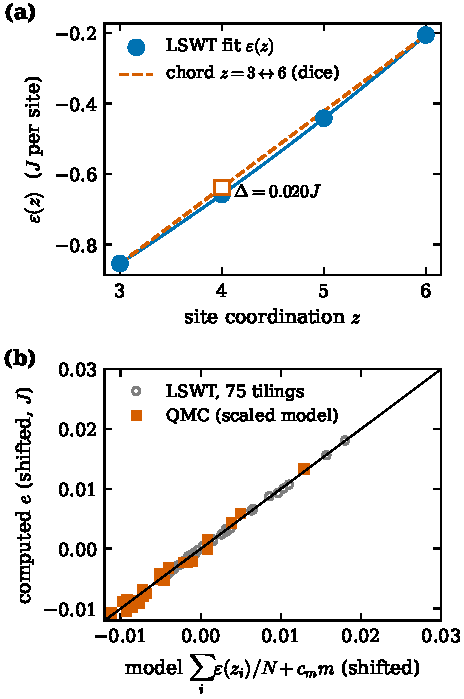
\includegraphics[width=\columnwidth]{figs/fig2_mechanism.pdf}
\caption{Coordination mechanism of quantum tiling selection ($S=\frac12$). (a)~Single-site zero-point energies $\eps(z)$ obtained by fitting LSWT energies of 75 tilings to Eq.~(\ref{eq:coord}). $\eps(z)$ is convex, so at fixed $\langle z\rangle=4$ the uniform $z=4$ tiling lies below the dice combination (open square) by $\Delta=0.020J$ per site. (b)~Energies computed for many tilings vs the coordination model: LSWT (open circles, rms residual $1.4\times10^{-4}J$) and QMC with the model rescaled linearly (squares, rms $5\times10^{-4}$--$8\times10^{-4}J$). Both axes are shifted by a common constant.}
\label{fig:mech}
\end{figure}

\subsection{A local, convex zero-point energy}

We first computed the LSWT energy of 75 tilings with widely different structure: tilt-family strips, and tilings with up to 200 random flips. Their energies are reproduced by a purely local form,
\begin{equation}
\frac{E_{\rm LSWT}}{N}\simeq\frac1N\sum_i\eps(z_i)+c_m\,m ,
\label{eq:coord}
\end{equation}
with $\eps(3,4,5,6)=(-0.8544,-0.6582,-0.4423,-0.2061)J$ and $c_m=0.0304J$ for $S=\frac12$. The rms residual is $1.4\times10^{-4}J$, compared with a spread of energies of $6.8\times10^{-3}J$ [Fig.~\ref{fig:mech}(b)]. The small $c_m$ term accounts for the weak cost of sublattice imbalance.

The key property is that $\eps(z)$ is \emph{convex} [Fig.~\ref{fig:mech}(a)]. Physically, a site with many neighbors has its quantum fluctuations shared among many bonds, so its zero-point energy per bond is smaller but its total is larger. Because $\sum_iz_i=4N$ is fixed for every tiling, Jensen's inequality gives
\begin{equation}
\frac1N\sum_i\eps(z_i)\;\ge\;\eps(\langle z\rangle)=\eps(4),
\label{eq:jensen}
\end{equation}
with equality only when all $z_i=4$. Every other tiling pays for its coordination variance. Tilings with all $z_i=4$ are not unique: besides the square-type tiling there are folded variants (Sec.~\ref{sec:geom}). As graphs, however, all of them are square lattices, so the zero-field ground state is in every case the square-lattice antiferromagnet. The dice lattice, whose coordinations $3,3,6$ lie farthest from 4, is the most expensive at $h=0$.

\emph{How good is the local model?} We tested Eq.~(\ref{eq:coord}) in four ways (Appendix~\ref{app:tests}). (i)~On an enlarged training set of 128 tilings ($L=18,24$, up to 600 random flips) the rms residual is $1.6\times10^{-4}J$ in leave-one-out cross-validation, with no systematic dependence on system size, number of flips or starting structure (largest class-averaged residual $1.8\times10^{-4}J$). (ii)~Adding the number of bonds of each type $(z_i,z_j)$ as extra terms halves the residual, to $0.9\times10^{-4}J$. Correlations between neighboring coordinations are therefore present but small. (iii)~Out of sample, on 71 periodic crystals evaluated with LSWT in the thermodynamic limit, the residual is $2.4\times10^{-4}J$ ($1.5\times10^{-4}J$ with pair terms). (iv)~Tilings with \emph{identical} coordination histograms but different arrangements differ by at most $3.5\times10^{-4}J$. The model therefore resolves differences of order $10^{-3}J$, such as the depth of the $\Md/2$ and $2\Md/3$ hull points, but not differences of order $10^{-4}J$. We use it only to screen candidates. Every energy on which a conclusion rests is computed with QMC.

QMC confirms this picture quantitatively. For $S=\frac12$ we find $e_0=-0.66917(30)J$ for the square-type and $-0.63786(30)J$ for the dice tiling, a difference of $0.0313J$ per site, compared with zero classically. The QMC energies of all structures studied, including strips, periodic crystals and annealed networks, follow the coordination model after a single linear rescaling, $e_{\rm QMC}=a+b\,e_{\rm model}$ with $b=1.27$, to $5$--$8\times10^{-4}J$ [Fig.~\ref{fig:mech}(b)]. This model is what makes the exhaustive searches of Sec.~\ref{sec:field} possible.



\subsection{The cost of a moment: why hubs are avoided}

Equation~(\ref{eq:coord}) also tells us how a tiling can acquire a moment most cheaply. On any bipartite tiling each bond joins $A$ to $B$, so $\sum_{i\in A}z_i=\sum_{i\in B}z_i=2N$. Writing $q_i=\pm(z_i-4)$, with $+$ on the minority sublattice $A$ and $-$ on $B$, this gives
\begin{equation}
m=\frac{N_B-N_A}{2N}=\frac1{8N}\sum_i q_i .
\label{eq:charge}
\end{equation}
Every site with $z\ne4$ thus carries a ``moment charge'' $q_i$, and the model assigns it the cost $\eps(z_i)-\eps(4)$. Because $\sum_i(z_i-4)=0$, charges come in neutral groups. The cheapest group is a $z=5$ site on $A$ with a $z=3$ site on $B$: charge $+2$ at cost $\eps(5)+\eps(3)-2\eps(4)=0.0197J$, i.e., $0.0099J$ per unit charge. A hub requires a $z=6$ site on $A$ and two $z=3$ sites on $B$: charge $+4$ at cost $\eps(6)+2\eps(3)-3\eps(4)=0.0597J$, i.e., $0.0149J$ per unit charge, 50\% more. To leading order, the energy therefore rises \emph{linearly} with $m$, with slope $8\times0.0099J$, as long as the moment can be carried by aligned $3/5$ pairs alone. It rises more steeply once hubs become unavoidable.

The largest moment that $3/5$ pairs can carry is fixed by the geometry of the tiling. In every supercell we enumerated completely (all 29 cells with up to 27 sites that fit an $L=36$ torus) and among all retained candidates in the 36-site cells, no hub-free tiling has $m>1/12$, i.e., $M>\Md/2$. (For the 36-site cells this rules out the cheapest hub-free tilings, with all $z=3$ sites on $B$ and all $z=5$ sites on $A$, because these have lower model energy than any tiling with hubs at the same $m$ and would have been retained. Hub-free tilings with misaligned $3/5$ sites are not excluded there, but they cost more.) The leading-order energy $e_{\rm model}(m)$ is therefore a straight line from the square-type tiling to the hub-free $\Md/2$ crystal, followed by a steeper segment to dice. The $\Md/2$ crystal sits at the kink between them. This gives two predictions, both borne out below. The $\Md/2$ plateau is robust, because it rests on the leading term. Structures with $0<M<\Md/2$ are nearly degenerate at leading order, so the low-field plateaus are decided by the smaller arrangement-dependent energies of Sec.~\ref{sec:zero}A and are correspondingly fragile.

\subsection{Tilt family and negative walls}

\begin{figure}[t]
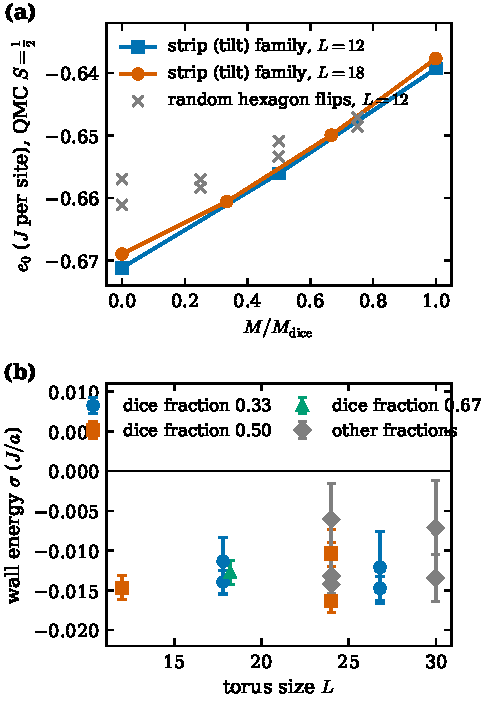
\includegraphics[width=\columnwidth]{figs/fig3_tilt_walls.pdf}
\caption{(a)~QMC ground-state energies ($S=\frac12$) of the tilt family (parallel strips of dice and square tiling) for $L=12$ and $18$, together with tilings obtained by random hexagon flips (crosses). Random flips cost energy at fixed $M$; the classical energy is $-0.5J$ for all points. (b)~Energy per unit length of a dice$|$square wall extracted from the strips, for several dice fractions and torus sizes. All values are negative.}
\label{fig:tilt}
\end{figure}

Figure~\ref{fig:tilt}(a) shows the QMC energy of the tilt family as a function of its moment. The curve is slightly concave: intermediate strip patterns lie \emph{below} the straight line joining the square-type and dice tilings. Subtracting the bulk energies gives the energy per unit length of a dice$|$square wall. It is negative for every width, fraction and system size studied, $\sigma\approx-0.011$ to $-0.015J/a$ [Fig.~\ref{fig:tilt}(b)]. The coordination picture explains the sign. A wall converts rim ($z=3$) and hub ($z=6$) sites of dice into $z=4,5$ sites, which lowers $\sum_i\eps(z_i)$ because $\eps$ is convex. By contrast, random flips at fixed $M$ (crosses) always raise the energy, in agreement with Ref.~\cite{Jagannathan2012}. The sign of $\sigma$ is also opposite to that of the phason-flip walls inside the SDL, whose line energy is $+0.062J/a$~\cite{Jagannathan2013}. Those walls separate two tilings with the same coordination histogram, so they cannot lower $\sum_i\eps(z_i)$; a dice$|$square wall can.

\begin{figure*}[t]
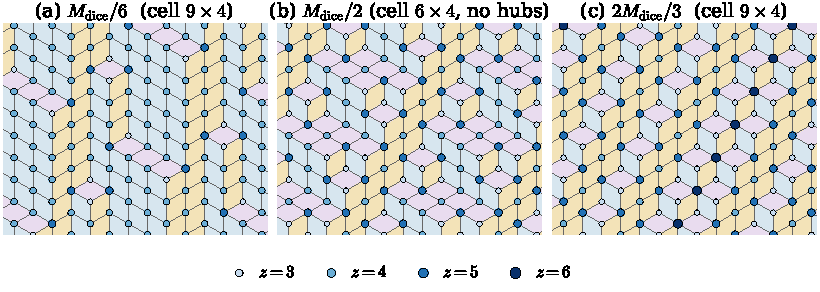
\includegraphics[width=\textwidth]{figs/fig4_crystals.pdf}
\caption{Periodic tilings on the lower convex hull of $e_0(m)$ (QMC, $S=\frac12$). (a)~$\Md/6$ crystal (cell $9\times4$, shear $s=5$): sparse $z=3,5$ pairs in a square-type background. (b)~$\Md/2$ crystal (cell $6\times4$, $s=4$): $z=3,4,5$ in equal numbers and \emph{no} sixfold hubs. (c)~$2\Md/3$ crystal (cell $9\times4$, $s=7$): the first appearance of hubs, $z_3{:}z_4{:}z_5{:}z_6=16{:}6{:}12{:}2$. Color code as in Fig.~\ref{fig:tilings}.}
\label{fig:crystals}
\end{figure*}

\begin{figure*}[t]
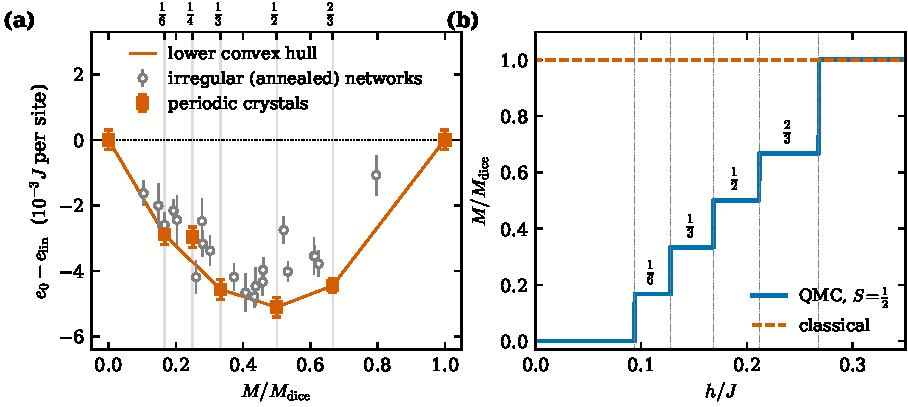
\includegraphics[width=\textwidth]{figs/fig5_staircase.pdf}
\caption{Magnetization staircase ($S=\frac12$, QMC). (a)~Zero-field energy relative to the straight line between the square-type and dice tilings, $e_{\rm lin}(m)=e_{\rm sq}+6m\,(e_{\rm dice}-e_{\rm sq})$. Squares: best periodic crystal at each $M/\Md$ (cells $\le36$ sites; $L=36$ for $\frac16,\frac13,\frac12,\frac23$, $L=24$ for $\frac14$). Circles: irregular networks from LSWT annealing at $L=18,24,30$. The line is the lower convex hull. (b)~$T=0$ magnetization obtained by minimizing $e_0-hm$ over the hull (solid), compared with the classical jump (dashed). Dotted vertical lines mark the step fields listed in Table~\ref{tab:crystals}.}
\label{fig:stair}
\end{figure*}

A negative wall energy has a direct consequence. When the field makes dice favorable, the system does not phase-separate into large dice and square domains. It instead gains energy by creating walls. In LSWT on $L=36$ and $48$ tori the energy per straight wall is $\sigma_\infty\approx-0.0088J/a$ for widely separated walls. It becomes about $0.0005J/a$ more negative when the walls are six rows apart, the closest spacing compatible with bipartiteness [Fig.~\ref{fig:A2}(b)]. Straight walls therefore attract at short distance. The wall picture explains why intermediate structures win, but it does not select the crystal. Superlattices of straight walls lie $2.0$--$2.5\times10^{-3}J$ above the best crystals at the same $m$ (LSWT at $m=1/18$, $1/12$ and $1/9$). The reason is their histogram: the straight-wall superlattice at $\Md/2$ still contains 8\% hubs, whereas the crystal has none. The selection is controlled by the coordination histogram, as in Sec.~\ref{sec:zero}B, and the negative wall energy is its consequence rather than an independent cause.

%=====================================================================
\section{Field-driven crystals and the magnetization staircase}\label{sec:field}
%=====================================================================




\begin{table*}[t]
\caption{Periodic crystals on or near the lower hull ($S=\frac12$). $M/\Md=6m$. Coordination counts are per cell. $\delta e=e_0-e_{\rm lin}$ from QMC, per site, with $L$ the torus size used. The last column gives the field window in which the crystal is the $T=0$ ground state.}
\label{tab:crystals}
\begin{ruledtabular}
\begin{tabular}{lccccc}
$M/\Md$ & cell $(p,q,s)$ & $z_3{:}z_4{:}z_5{:}z_6$ & $\delta e$ ($10^{-3}J$) & $L$ & window ($h/J$)\\
\hline
0 & square & $0{:}1{:}0{:}0$ & 0 & 24 & $<0.094$\\
$\frac16$ & $(9,4,5)$ & $4{:}28{:}4{:}0$ & $-2.90(10)$ & 36 & $0.094$--$0.128$\\
$\frac14$ & $(4,6,0)$ & $5{:}14{:}5{:}0$ & $-2.97(31)$ & 24 & ---\\
$\frac13$ & $(3,12,0)$ & $8{:}20{:}8{:}0$ & $-4.57(13)$ & 36 & $0.128$--$0.168$\footnotemark[1]\\
$\frac12$ & $(6,4,4)$ & $8{:}8{:}8{:}0$ & $-5.11(10)$ & 36 & $0.168$--$0.212$\\
$\frac23$ & $(9,4,7)$ & $16{:}6{:}12{:}2$ & $-4.45(10)$ & 36 & $0.212$--$0.268$\\
1 & dice & $2{:}0{:}0{:}1$ & 0 & 24 & $>0.268$\\
\end{tabular}
\end{ruledtabular}
\footnotetext[1]{The same structure gives $-3.8(3)$ at $L=24$, and a different $\frac13$ structure gives $-4.06(53)$ at $L=18$.}
\end{table*}

\subsection{Exhaustive search of periodic tilings}

Because the energy of a tiling is essentially a function of its coordination histogram, we can scan the complete set of periodic tilings with small unit cells. For all supercells with up to 36 sites we enumerated every tiling ($2.6$--$5.4\times10^5$ per cell for the 36-site cells), retained the bipartite ones, and kept the lowest four to six at each $m$ according to Eq.~(\ref{eq:coord}). For cells with up to 27 sites we also re-ranked with LSWT \emph{every} tiling within $1.5\times10^{-3}J$ of the model minimum at the $m$ values of the hull. The survivors were ranked with LSWT in the thermodynamic limit (a Bloch calculation on the supercell, which agrees with $L=36$ tori to $10^{-8}J$), and the best ones evaluated with QMC. In a 36-site cell the imbalance $N_A-N_B$ is even, so $m$ takes only the values $k/36$, i.e., $M/\Md=k/6$. The enlarged cells therefore do not create new values of $M/\Md$. They do, however, uncover lower-energy structures at existing values, which is how the $\Md/6$ and $2\Md/3$ crystals were found.

Figure~\ref{fig:crystals} shows the crystals that lie on the lower convex hull, and Fig.~\ref{fig:stair}(a) and Table~\ref{tab:crystals} give their energies. Three features stand out.

(1)~The deepest point of the hull is the $\Md/2$ crystal, $\delta e=-5.11(10)\times10^{-3}J$ at $L=36$ [$-5.4(4)\times10^{-3}J$ at $L=24$]. Remarkably, it contains \emph{no} hubs. Its sites have $z=3,4,5$ in equal numbers. The crystal is thus the closest one can come to the dice moment while keeping every coordination adjacent to 4, which is exactly what a convex $\eps(z)$ rewards. It has the same coordination histogram as the compensated SDL of Refs.~\cite{Jagannathan2012,Jagannathan2013}. The difference is the arrangement: in the $\Md/2$ crystal the arrangement places the surplus sites on one sublattice, giving $m=1/12$ instead of $0$. The comparison also provides an independent check of Eq.~(\ref{eq:coord}). For the SDL it predicts $E_{\rm LSWT}/N=[\eps(3)+\eps(4)+\eps(5)]/3=-0.6516J$, in agreement with the value $-0.6517(7)J$ obtained by direct LSWT in Ref.~\cite{Jagannathan2013}. The QMC energy of the SDL, $-0.6639J$~\cite{Jagannathan2012}, lies $5.3\times10^{-3}J$ above our square-type value, again as Jensen's inequality requires.

(2)~The $2\Md/3$ crystal, $\delta e=-4.45(10)\times10^{-3}J$, lies $1.0\times10^{-3}J$ below the chord between the $\Md/2$ crystal and dice, about ten statistical errors. It is the first hull structure that contains hubs, but only one site in 18.

(3)~At low moment the $\Md/6$ crystal, a dilute array of $z=3$/$z=5$ pairs in a square background, lies $0.6\times10^{-3}J$ below the chord from $m=0$ to $\Md/3$. The $\Md/3$ crystal, evaluated at $L=36$, lies $0.56\times10^{-3}J$ below the chord between $\Md/6$ and $\Md/2$. The $\Md/4$ structure is above the hull.

Irregular networks produced by annealing (gray circles) never reach the hull. They come from 55 LSWT-driven annealing runs at $L=18$ and 106 two-stage (model, then LSWT) runs at $L=24$ and $30$. The runs spanned five tilt sectors, fields $0$--$0.3J$ and two to three random seeds per setting. The best of them, near $M/\Md\approx0.4$--$0.5$, have $\delta e\approx-4.5\times10^{-3}J$, about $0.6\times10^{-3}J$ above the $\Md/2$ crystal. As anticipated, the ground state in a field is a symmetric crystal, not a disordered network.

\subsection{Staircase}

At $T=0$ the tiling selected by a field $h$ minimizes $e_0(m)-hm$, with $-\frac12\chi h^2$ added for the compensated tiling. Minimizing over the hull yields the staircase of Fig.~\ref{fig:stair}(b):
\begin{equation*}
0\xrightarrow{0.094}\tfrac16\xrightarrow{0.128}\tfrac13\xrightarrow{0.168}\tfrac12\xrightarrow{0.212}\tfrac23\xrightarrow{0.268}1,
\end{equation*}
with step fields in units of $J$ and magnetization in units of $\Md$. The classical jump at $h=0^+$ is thus replaced by four plateaus between $h=0.094J$ and $0.268J$, of widths $0.034$, $0.040$, $0.044$ and $0.056J$. This staircase is established within the searched space: periodic cells with up to 36 sites plus the annealed networks. It is not a proof over all tilings. The deepest point of the hull is the hub-free $\Md/2$ crystal. The widest plateau belongs to its neighbor at $2\Md/3$, which has a hub on one site in 18. Each step corresponds to a first-order change of the \emph{lattice} and not only of the spin state.

\emph{Robustness.} We assess the staircase in three ways. (i)~\emph{Statistical errors.} Resampling all QMC energies within their errors (4000 samples, Table~\ref{tab:robust}) keeps the $2\Md/3$ plateau in essentially all samples, the $\Md/2$ and $\Md/3$ plateaus in 95\% and 94\%, and the $\Md/6$ plateau in 86\%. The $\Md/3$ result depends on system size, however. The same structure gives $-4.57(13)\times10^{-3}J$ at $L=36$ but $-3.8(3)\times10^{-3}J$ at $L=24$, and with the $L=24$ value it would lie on the chord. We use the larger system, and we regard the $\Md/3$ and $\Md/6$ plateaus, which rest on sub-$10^{-3}J$ margins, as less secure than $\Md/2$ and $2\Md/3$. (ii)~\emph{System size.} The $\Md/2$ deviation is $-4.8$, $-5.4(4)$ and $-5.11(10)\times10^{-3}J$ at $L=12$, $24$ and $36$. The square-type and dice references agree between $L=18$ and $24$ to $10^{-4}J$. In LSWT the crystal energies at $L=36$ coincide with the thermodynamic limit. (iii)~\emph{Cell size.} In LSWT the best $\Md/3$ energy changes by only about $10^{-4}J$ between 9- and 36-site cells, and the best $\Md/2$ structure already appears in 24-site cells. The $\Md/6$ crystal needs at least 36 sites per cell, and the $2\Md/3$ optimum also first appears there. For $2\Md/3$ the energy drops by $1.9\times10^{-3}J$ from 18- to 36-site cells. Convergence in cell size is therefore not demonstrated for these two plateaus, and larger cells may lower them further or add new steps nearby. Lowering an existing hull point cannot remove it from the hull, but a new structure at a nearby $m$ could. The leading-order analysis of Sec.~\ref{sec:zero}B suggests that the $\Md/2$ kink is protected, and that additional steps, if any, are most likely below $h\approx0.17J$, where the leading-order energy is linear.

\begin{table}[t]
\caption{Robustness of the staircase to the QMC statistical errors: fraction of 4000 resampled hulls in which each plateau appears, and mean and standard deviation of the step fields (in $J$).}
\label{tab:robust}
\begin{ruledtabular}
\begin{tabular}{lcc}
plateau $M/\Md$ & present & lower edge $h/J$\\
\hline
$\frac16$ & 0.86 & $0.090\pm0.016$\\
$\frac14$ & 0.02 & ---\\
$\frac13$ & 0.94 & $0.129\pm0.012$\\
$\frac12$ & 0.95 & $0.169\pm0.013$\footnotemark[1]\\
$\frac23$ & 1.00 & $0.212\pm0.012$\\
1 (dice) & 1.00 & $0.268\pm0.007$\\
\end{tabular}
\end{ruledtabular}
\footnotetext[1]{When the $\frac13$ plateau is present; otherwise $0.149\pm0.007$.}
\end{table} Within each plateau the spin ground state is pinned at $S_{\rm tot}=M$, as required by Lieb's theorem, because $S^z_{\rm tot}$ is conserved on a fixed graph.

%=====================================================================
\section{Fluctuations, entanglement and spectroscopic signatures}\label{sec:fluct}
%=====================================================================

\begin{figure}[t]
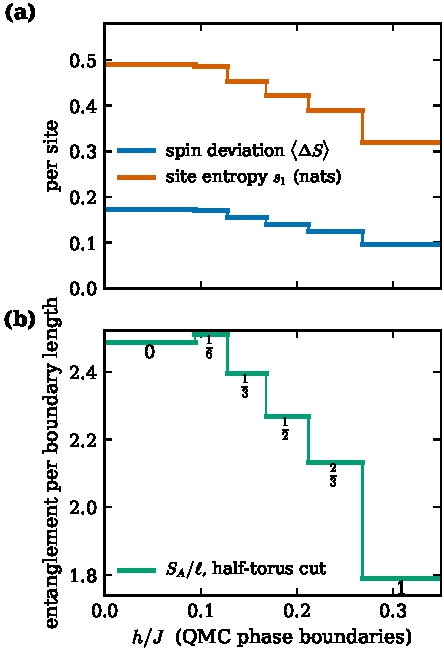
\includegraphics[width=\columnwidth]{figs/fig6_fluct.pdf}
\caption{Quantum-fluctuation measures of the LSWT ground state ($S=\frac12$, $L=36$) of the crystal selected at each field, using the QMC phase boundaries. (a)~Mean spin deviation $\langle\Delta S\rangle=\langle a^\dagger a\rangle$ and single-site entanglement entropy. (b)~Gaussian entanglement entropy of half the torus per unit boundary length. Plateau labels give $M/\Md$.}
\label{fig:fluct}
\end{figure}

\begin{figure*}[t]
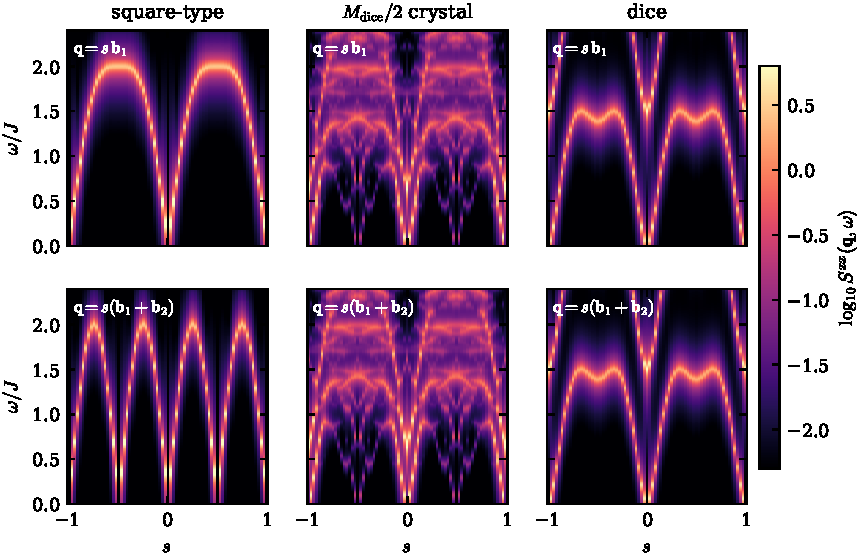
\includegraphics[width=\textwidth]{figs/fig7_sqw.pdf}
\caption{LSWT transverse dynamical structure factor $\log_{10}S^{xx}(\mathbf q,\omega)$ ($S=\frac12$, $L=36$, Lorentzian broadening $0.03J$) along $\mathbf q=s\,\mathbf b_1$ (top) and $\mathbf q=s(\mathbf b_1+\mathbf b_2)$ (bottom), where $\mathbf b_{1,2}$ are the reciprocal vectors of the triangular lattice. Left: square-type tiling (a single sharp magnon branch). Center: $\Md/2$ crystal (backfolded minibands and gaps set by the $6\times4$ cell). Right: dice (a Goldstone branch plus the dispersionless band near $1.5J$ that comes from the rim sites).}
\label{fig:sqw}
\end{figure*}

Because the spin state within a plateau does not change with $h$, the quantum-fluctuation content of the ground state changes only at the steps, where the lattice changes. Figure~\ref{fig:fluct} follows three measures along the staircase. The mean spin deviation decreases from $0.173$ (square-type) through $0.171$, $0.154$, $0.140$ and $0.124$ to $0.095$ (dice), and the single-site entanglement entropy falls from $0.49$ to $0.32$. The half-system entanglement per unit boundary length first rises slightly at the $\Md/6$ step and then drops by $28\%$ between the square-type and dice tilings. The field thus reduces quantum fluctuations in discrete steps, by selecting lattices with more low-coordination sites whose moments are more nearly classical. This is the mirror image of the zero-field selection.

The crystals can be distinguished spectroscopically [Fig.~\ref{fig:sqw}]. The square-type tiling shows a single linear-dispersing magnon branch. The dice tiling combines a Goldstone branch with the dispersionless band near $\omega\approx1.5J$ localized on the rims~\cite{Sutherland1986,Vidal1998}. The $\Md/2$ crystal shows backfolded minibands with small gaps at the zone boundaries of its $6\times4$ cell. Its low-energy branch is square-like, and its upper spectral weight is spread over a band of nearly flat modes. These features give a direct fingerprint of each plateau in inelastic neutron scattering or in magnon spectroscopy of engineered structures.

%=====================================================================
\section{Dependence on spin length}\label{sec:spinS}
%=====================================================================

\begin{figure}[t]
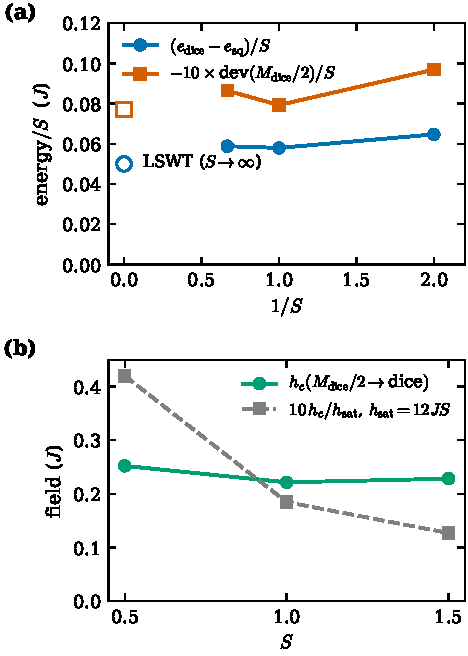
\includegraphics[width=\columnwidth]{figs/fig8_spinS.pdf}
\caption{Spin-$S$ QMC ($L=12$, $\beta JS=12$). (a)~Selection energies per unit $S$: dice minus square-type (circles) and the $\Md/2$ deviation (squares, $\times10$). Open symbols: LSWT ($S\to\infty$). Both approach finite limits, i.e., selection energies scale as $JS$. (b)~The field at which the $\Md/2$ crystal gives way to dice at this system size (circles) is $S$-independent in units of $J$. Relative to the saturation scale, the intermediate region therefore shrinks as $1/S$ (squares).}
\label{fig:spinS}
\end{figure}

\begin{table}[b]
\caption{Spin-$S$ dependence (QMC, $L=12$). Energies per site in units of $J$.}
\label{tab:spinS}
\begin{ruledtabular}
\begin{tabular}{lccc}
$S$ & $(e_{\rm dice}-e_{\rm sq})/S$ & $\delta e(\Md/2)/S$ & $h_c(\Md/2\to{\rm dice})$\\
\hline
$\frac12$ & 0.065 & $-0.0097$ & 0.25\\
1 & 0.058 & $-0.0079$ & 0.22\\
$\frac32$ & 0.059 & $-0.0086$ & 0.23\\
LSWT & 0.050 & $-0.0077$ & ---\\
\end{tabular}
\end{ruledtabular}
\end{table}

Classically the selection energy vanishes, and in spin-wave theory it is of order $JS$, whereas the exchange energy is of order $JS^2$. QMC for $S=\frac12$, $1$ and $\frac32$ confirms this scaling (Fig.~\ref{fig:spinS} and Table~\ref{tab:spinS}). The ratios $(e_{\rm dice}-e_{\rm sq})/S$ and $\delta e(\Md/2)/S$ are nearly constant and extrapolate to the LSWT values. Both the energy differences and the Zeeman energy $hM\propto hS$ are linear in $S$, so the step fields are $S$-independent in units of $J$. The field at which the $\Md/2$ crystal gives way to dice is $0.22$--$0.25J$ for all three spins. Measured against the saturation field of order $12JS$, the intermediate region therefore shrinks as $1/S$. The staircase is a genuinely quantum phenomenon, most pronounced for $S=\frac12$, but it survives for all $S$ at fixed $h/J$.

%=====================================================================
\section{Finite temperature in an effective tiling model}\label{sec:finiteT}
%=====================================================================

\begin{figure}[t]
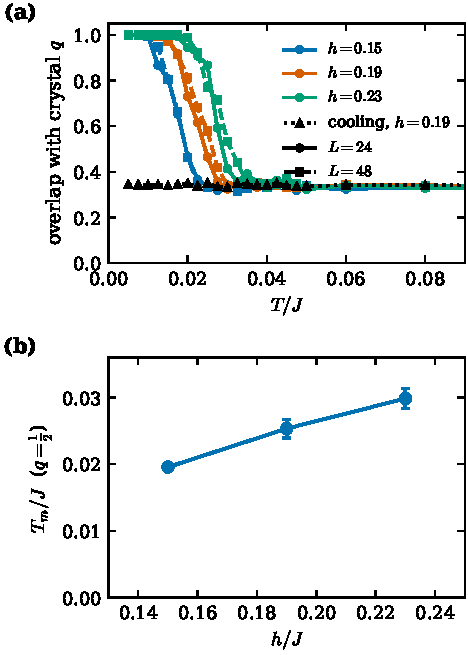
\includegraphics[width=\columnwidth]{figs/fig9_melting.pdf}
\caption{Thermal stability of the $\Md/2$ crystal (tiling Monte Carlo with the QMC-scaled coordination model, local hexagon flips, crystal tilt sector). (a)~Overlap $q$ of the tiling with the crystal on heating for three fields and two sizes, and on slow cooling from the disordered state (triangles). $q\simeq\frac13$ is the value for an uncorrelated tiling. (b)~Melting temperature, defined by $q=\frac12$.}
\label{fig:melt}
\end{figure}

When the tiling can rearrange, for example during growth, self-assembly or in a programmable array, the plateau crystals compete with the configurational entropy of the tiling. We model this with the QMC-scaled coordination free energy and local hexagon flips in the crystal's tilt sector. The spins are not sampled thermally. The temperatures below are therefore melting scales of this effective model, not transition temperatures of the full spin-plus-tiling system. Heating the $\Md/2$ crystal at fixed field [Fig.~\ref{fig:melt}(a)] produces a sharp loss of crystalline overlap at $T_m=0.020$, $0.025$ and $0.030J$ for $h=0.15$, $0.19$ and $0.23J$. The results for $L=24$ and $48$ coincide. $T_m$ increases with $h$ [Fig.~\ref{fig:melt}(b)] because the field deepens the hull minimum at $\Md/2$. On slow cooling from the disordered state, however, the system does not recrystallize. The overlap remains at the random value and the magnetization freezes near $0.47\Md$. Cooling 50 times more slowly does not change this [Fig.~\ref{fig:A2}(c)]. The final state has $G=e_0-hm$ higher than the crystal by $0.9$--$1.3\times10^{-3}J$ per site. It is therefore a metastable state of the local-flip dynamics, i.e., kinetic trapping, and not evidence for an equilibrium glass phase. This trapping is a practical consideration for any realization in which the tiling is annealed.

Two omitted effects can be estimated. (i)~\emph{Magnon entropy.} From Bloch LSWT, the magnon free energy per site of the crystals at $T=0.02$--$0.03J$ is $-1.6\times10^{-6}$ (square-type) to $-7\times10^{-5}J$ (dice), roughly proportional to $m$. On melting at $h=0.19J$ the magnetization drops by $\Delta m\approx0.018$ and the configurational entropy rises by $\Delta s\approx0.1$ per site. The magnon correction shifts $T_m$ by about $\Delta F_{\rm mag}/\Delta s\sim10^{-4}J$ and the step fields by $\lesssim5\times10^{-4}J$, both negligible. (ii)~\emph{Tilt-changing moves} enlarge the configuration space of the disordered state but not of the locked crystal. They would therefore lower $T_m$, so our values are best read as upper estimates within this model. A joint treatment of spin and tiling fluctuations is left for future work.

%=====================================================================
\section{Geometric interpretation: folded and crumpled surfaces}\label{sec:geom}
%=====================================================================

\begin{figure*}[t]
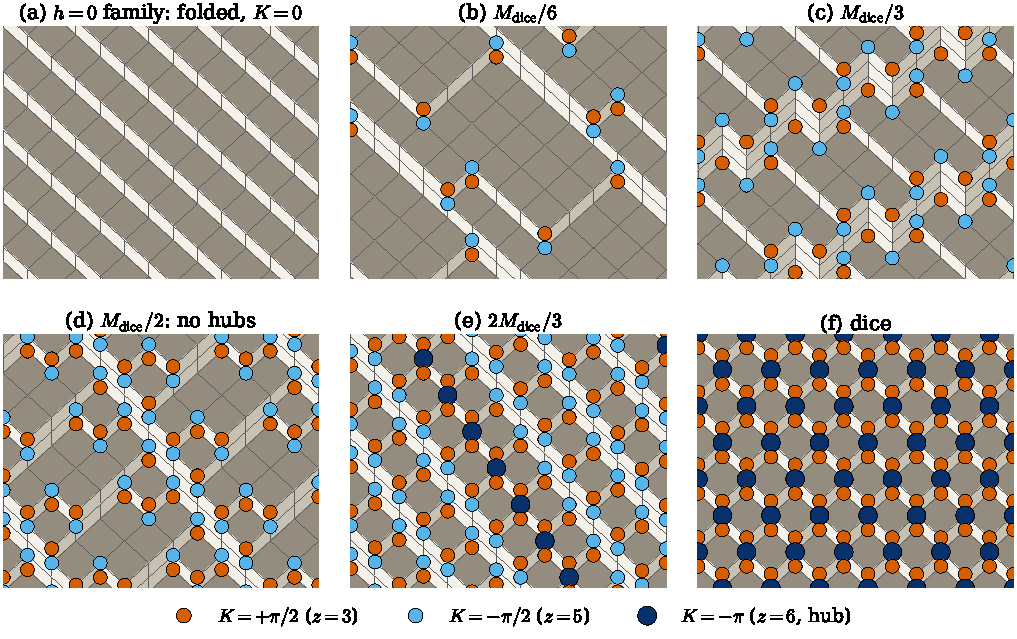
\includegraphics[width=\textwidth]{figs/fig10_curvature.pdf}
\caption{Tilings lifted to stepped surfaces in $\mathbb Z^3$ (orthographic view, tilted by $12^\circ$ from $[111]$; faces shaded by orientation). Colored dots mark vertices with nonzero discrete Gaussian curvature $K_i=2\pi-\frac\pi2 z_i$. (a)~A zero-curvature tiling from the degenerate $h=0$ family: two facets joined by straight folds, $K_i=0$ everywhere. (b)--(e)~The plateau crystals. Positive curvature ($z=3$) sits only on the majority sublattice and negative curvature ($z=5,6$) only on the minority sublattice. The $\Md/2$ crystal (d) uses only $\pm\pi/2$ vertices. (f)~Dice: $+\pi/2$ cones and $-\pi$ hubs.}
\label{fig:curv}
\end{figure*}

\emph{Definitions.} Every lozenge tiling is the projection along $[111]$ of a stepped surface $\Sigma$ made of unit squares of the cubic lattice~\cite{Kenyon2006}. We lift the tiling by assigning the steps $+\mathbf e_x$, $+\mathbf e_y$, $+\mathbf e_z$ to the bond directions $\mathbf a_1$, $\mathbf a_2-\mathbf a_1$, $-\mathbf a_2$ (whose sum vanishes). Each lozenge becomes a unit square face, and the tiling graph becomes the edge skeleton of $\Sigma$. We verified that the lift is single-valued for all structures shown. Around a vertex of coordination $z_i$ there are exactly $z_i$ faces, each contributing a right angle, so the discrete Gaussian curvature (angle deficit) is
\begin{equation}
K_i=2\pi-\frac{\pi}{2}\,z_i=\tfrac{\pi}{2}\,(4-z_i).
\label{eq:K}
\end{equation}
Sites with $z=3,4,5,6$ are cones ($+\pi/2$), flat points ($0$), saddles ($-\pi/2$) and strong saddles ($-\pi$). Two exact identities follow. First, $\langle z\rangle=4$ is the discrete Gauss--Bonnet theorem on the torus, $\sum_iK_i=0$. Second, inserting Eq.~(\ref{eq:K}) into Eq.~(\ref{eq:charge}) gives
\begin{equation}
N_B-N_A=-\frac{1}{2\pi}\sum_i\eta_iK_i,\qquad S_{\rm tot}=\frac{S}{2\pi}\Big|\sum_i\eta_iK_i\Big| ,
\label{eq:stagK}
\end{equation}
with $\eta_i=+1$ ($-1$) on sublattice $A$ ($B$). The total curvature always vanishes, and the Lieb moment is its sublattice-staggered part. We checked Eq.~(\ref{eq:stagK}) numerically for every structure in Fig.~\ref{fig:curv}. We distinguish this local quantity from the \emph{tilt}, the average orientation of $\Sigma$. The tilt is fixed by the fractions of the three lozenge orientations and is conserved by hexagon flips.

\emph{The results in this language.} (i)~Because $z_i$ is linear in $K_i$, Eq.~(\ref{eq:coord}) states that the quantum zero-point energy is, to leading order, a convex function of the local Gaussian curvature. At zero field it is minimized by surfaces with $K_i=0$ everywhere. These are not only the flat facet (the square-type tiling) but also facets joined by straight folds along cube axes [Fig.~\ref{fig:curv}(a)], i.e., developable, origami-like surfaces. All of them are square lattices as graphs (every vertex has degree 4 and every face is a quadrilateral), so their Hamiltonians coincide in the bulk. Consistently, the 68 distinct zero-curvature crystals (cell, orientation) in our enumeration have thermodynamic-limit LSWT energies within $2.5\times10^{-6}J$ of each other, a spread attributable to the finite $k$ grid. Folding costs nothing; curvature does. (ii)~By Eq.~(\ref{eq:stagK}) the Zeeman energy $-hS_{\rm tot}$ couples to staggered curvature. The field therefore crumples the surface, placing cones on the majority sublattice and saddles on the minority one. Every crystal on the hull is \emph{perfectly sorted}, $\sum_i|K_i|=|\sum_i\eta_iK_i|$: the mean $|K_i|$ is $20^\circ$, $40^\circ$, $60^\circ$, $80^\circ$ and $120^\circ$ for $M/\Md=\frac16,\frac13,\frac12,\frac23,1$, i.e., exactly $120^\circ\times M/\Md$. No curvature is wasted on the wrong sublattice. (iii)~The hub-free kink of Sec.~\ref{sec:zero}B reads: staggered curvature is cheapest in $\pm\pi/2$ vertices, $-\pi$ saddles cost 50\% more per unit, and the $\Md/2$ crystal is the densest packing of $\pm\pi/2$ vertices we find. (iv)~The field does \emph{not} control the tilt. The $\Md/3$, $\Md/2$ and dice surfaces all have the $[111]$ orientation, whereas the $\Md/6$ and $2\Md/3$ crystals found are tilted by $29^\circ$ and $25^\circ$, and the $h=0$ family contains orientations from $35^\circ$ to $55^\circ$. Bending of the average surface and crumpling are distinct, and only the latter carries the moment.

\emph{Limitations of the picture.} (a)~$\Sigma$ lives in an auxiliary height space. Its third dimension encodes connectivity and is not a physical displacement. Nothing here implies that a material buckles, unless the height is itself physical, which we do not assume. (b)~The analogy with origami is exact only for the zero-field family, whose folds keep $K_i=0$. The field-induced structures contain conical defects, so they are ``crumpled with cones'' rather than isometrically folded. There are no fold angles, rigidity or mechanics: all faces are unit squares with fixed right angles. (c)~The energy is not an elastic bending energy. It is a sum of local curvature costs $\eps(z_i)$ with small neighbor corrections ($\lesssim10^{-4}J$), and there is no metric or bending modulus. The convexity is a numerical result of LSWT and QMC for $S=\frac12$ to $\frac32$, not a consequence of geometry. (d)~Equations~(\ref{eq:K}) and (\ref{eq:stagK}) and Gauss--Bonnet are exact. Statements about energies inherit the accuracy of the coordination model and of QMC discussed above. (e)~The Legendre construction that turns $e_0(m)$ into the staircase is formally the same as the construction of faceted equilibrium crystal shapes. Here, however, $m$ is a staggered curvature density and not a surface orientation, so this analogy is structural only. (f)~On the torus the tilt is fixed by the boundary conditions. The tilts quoted in (iv) are those of the optimal cells found and may be one of several nearly degenerate variants.

%=====================================================================
\section{Discussion}\label{sec:disc}
%=====================================================================

\emph{Height-model interpretation.} Section~\ref{sec:geom} makes the height representation concrete: Eq.~(\ref{eq:coord}) is an effective height model whose potential is a convex function of the local Gaussian curvature of the lifted surface. The field acts as a chemical potential for the sublattice imbalance. In this language the plateaus are \emph{locked} phases of the height model, commensurate crystals analogous to the ordered phases of quantum dimer models~\cite{Rokhsar1988,Moessner2001}. The staircase is analogous to the devil's staircases of competing-interaction systems~\cite{Bak1982}, but here the underlying potential is set by the convexity of $\eps(z)$ and not by an imposed long-range interaction. Our data establish a finite set of steps. Whether the steps continue to subdivide in larger cells, particularly at low field where the hull is nearly straight (Table~\ref{tab:crystals}), is an open question.

\emph{Relation to known plateaus.} Magnetization plateaus in quantum magnets usually arise from a crystal of magnetic excitations on a \emph{fixed} lattice~\cite{Kageyama1999,Honecker2004}. Here the plateau is a crystal of the lattice itself, and the spin state on each plateau is the Lieb ground state of that lattice. The two mechanisms could coexist if bond strengths are also varied. Studying that would require going beyond the uniform-$J$ model~(\ref{eq:H}).

\emph{Platforms.} Three classes of system make the graph of exchange bonds a design or growth variable. (i)~\emph{$\pi$-magnetic nanographenes}, in which sublattice imbalance controls the ground-state spin in accordance with Lieb's theorem and the building blocks can be fused into extended networks~\cite{Mishra2020}. (ii)~\emph{Atom-by-atom spin arrays} on surfaces, which realize arbitrary two-dimensional coupling graphs and allow local spectroscopy of spin excitations~\cite{Khajetoorians2019}. (iii)~\emph{Programmable quantum simulators}, such as Rydberg arrays, in which the connectivity is reconfigurable and antiferromagnetic correlations on hundreds of sites have been measured~\cite{Scholl2021}. In (ii) and (iii) the energies $e_0(m)$ of different tilings can be compared directly, and the $\Md/2$ crystal is a concrete target structure. In (i) the step fields, $0.1$--$0.3J$, and the melting temperature, $0.02$--$0.03J$, give the relevant scales once $J$ is known.

\emph{Limitations.} (a)~The crystal search is exhaustive only for cells with up to 36 sites, and cell-size convergence is demonstrated for $\Md/3$ and $\Md/2$ but not for $\Md/6$ and $2\Md/3$. Larger cells may add steps or shift boundaries, most likely at low field. (b)~The $\Md/6$ and $\Md/3$ plateaus rest on margins of $0.6\times10^{-3}J$, and the $\Md/3$ margin changes between $L=24$ and $L=36$. (c)~The coordination model is used only for screening; its arrangement-dependent residual ($\lesssim3.5\times10^{-4}J$) is comparable to the energy differences that decide the low-field plateaus. (d)~The finite-temperature results refer to an effective tiling model at fixed tilt without thermal spin fluctuations. The quoted $T_m$ is a scale of that model, and the non-recrystallization is kinetic trapping. (e)~Irregular networks were generated with a model-assisted annealing that is not exhaustive. Every irregular network we evaluated with QMC lies above the periodic hull.

%=====================================================================
\section{Conclusion}\label{sec:concl}
%=====================================================================

We have shown that the classically degenerate family of lozenge-tiling networks is organized, quantum mechanically, by one simple rule: the zero-point energy is a convex function of the site coordination. This rule selects the uniform square-type tiling at zero field, makes dice$|$square walls attractive rather than costly, and, in competition with the Zeeman energy of the Lieb moment, stabilizes, within the searched space, a staircase of periodic crystals rather than the classical jump or a disordered network. Because a moment is carried most cheaply by pairs of $z=3$ and $z=5$ sites, the densest hub-free tiling, the $\Md/2$ crystal, is a kink of the leading-order energy. It is the central new object. It is stable over $0.168J<h<0.212J$ for $S=\frac12$, within a staircase of $\Md/6$, $\Md/3$, $\Md/2$ and $2\Md/3$ crystals. In an effective tiling model it melts at $T\simeq0.02$--$0.03J$. Its field window is $S$-independent in units of $J$. Geometrically, zero field selects folded, curvature-free surfaces, and the field crumples them with sorted conical defects, because the Lieb moment is exactly the sublattice-staggered Gaussian curvature. These results identify quantum order by disorder acting on the geometry of the exchange network itself. They also provide concrete target structures and energy scales for nanographene networks, atom-by-atom spin arrays and quantum simulators, in which that geometry can be designed.

\clearpage
\begin{acknowledgments}
We acknowledge helpful discussions. [Funding information to be added.]
\end{acknowledgments}

\appendix

%=====================================================================
\section{Spin-wave hull and finite-size effects}\label{app:lswt}
%=====================================================================

\begin{figure}[h!]
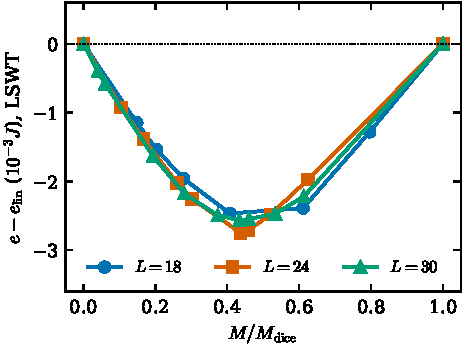
\includegraphics[width=\columnwidth]{figs/figA1_lswt_L.pdf}
\caption{LSWT energies of annealed tilings relative to the square-to-dice line for $L=18$, $24$, $30$. The lower envelope is size-independent to within $3\times10^{-4}J$.}
\label{fig:A1}
\end{figure}

The LSWT energies of the annealed tilings relative to the linear interpolation are independent of system size for $L=18$--$30$ (Fig.~\ref{fig:A1}). This justifies the use of $L\le36$ tori. LSWT underestimates the QMC deviations by a factor of about $1.3$ and the step fields by a factor of about $1.25$. It reproduces the ordering of the hull structures, but not differences below about $10^{-4}J$ (Appendix~\ref{app:tests}). For periodic crystals we also evaluate LSWT directly in the thermodynamic limit by Bloch diagonalization of the supercell ($6\times6$ to $64\times64$ $k$ points). For the crystals checked it agrees with $L=36$ tori to $10^{-8}J$. The $\Md/2$ crystal is the deepest LSWT hull point as well ($-3.7\times10^{-3}J$ at $L=36$).

%=====================================================================
\section{Tests of the coordination model, the wall picture and the cooling dynamics}\label{app:tests}
%=====================================================================

\begin{figure*}[t]
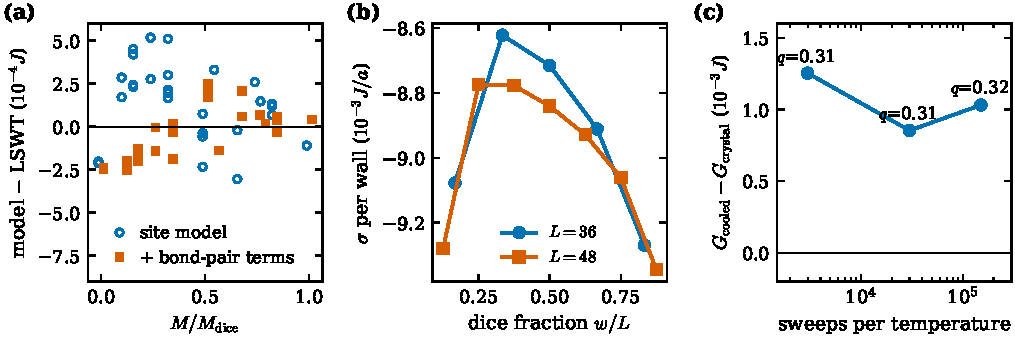
\includegraphics[width=\textwidth]{figs/figA2_tests.pdf}
\caption{(a)~Out-of-sample test of Eq.~(\ref{eq:coord}) on 71 periodic crystals, relative to thermodynamic-limit LSWT: site model (circles) and site model with bond-pair terms (squares). Points are offset horizontally for clarity. (b)~LSWT energy per straight dice$|$square wall for a dice strip of width $w$ in a square background on $L=36$ and $48$ tori. The walls are $w$ and $L-w$ rows apart, and closely spaced walls ($w/L$ near 0 or 1) have lower energy. (c)~Free energy $G=e_0-hm$ of the state reached by cooling to $T=0.005J$ relative to the $\Md/2$ crystal, for three cooling rates; labels give the overlap $q$ with the crystal.}
\label{fig:A2}
\end{figure*}

\emph{Coordination model.} The training set comprises the tilt family (dice, square-type, strips of width 6 and 12, and the $s6d3$ superlattice) at $L=18$ and $24$, each with 0 to 600 random hexagon flips, 128 tilings in total. The site model, Eq.~(\ref{eq:coord}), gives an rms residual of $1.55\times10^{-4}J$ ($1.60\times10^{-4}J$ leave-one-out). The largest single residual is $4.1\times10^{-4}J$. Residuals averaged over each class of starting structure and over each number of flips are below $1.8\times10^{-4}J$ and show no trend with the number of flips. Adding the densities of the ten bond types $(z_i,z_j)$ reduces the rms residual to $0.82\times10^{-4}J$ ($0.87\times10^{-4}J$ leave-one-out). The out-of-sample test on 71 periodic crystals [Fig.~\ref{fig:A2}(a)] gives $2.4\times10^{-4}J$ for the site model and $1.5\times10^{-4}J$ with pair terms. Within groups of crystals that share the same $m$ and the same histogram, LSWT energies differ by up to $3.5\times10^{-4}J$ (at $\Md/3$) and $3.1\times10^{-4}J$ (at $\Md/2$). The Spearman rank correlation between the pair model and LSWT within each $m$ is $0.76$--$0.92$. For the two $\Md/2$ structures evaluated with both methods, LSWT ($-0.64945$ vs $-0.64914J$) and QMC ($\delta e=-5.4(4)$ vs $-4.9(4)\times10^{-3}J$ at $L=24$) give the same order. For the two $\Md/3$ structures, LSWT separates them by $2.5\times10^{-4}J$. The LSWT-preferred one is also lower in QMC at $L=36$ [$-4.57(13)$ vs $-4.06(53)\times10^{-3}J$ at $L=18$], but its own value at $L=24$, $-3.8(3)\times10^{-3}J$, is not. Differences at the $10^{-4}J$ level are therefore not reliably ranked.

\emph{Walls.} Straight-wall superlattices at $m=1/18$, $1/12$ and $1/9$ have LSWT energies $-0.65076$, $-0.64718$ and $-0.64246J$, compared with $-0.65281$, $-0.64945$ and $-0.64492J$ for the best crystals. Their histograms contain 6\%, 8\% and 17\% hubs, respectively.

\emph{Cooling.} Starting from the melted state at $T=0.05J$ and cooling to $0.005J$ in 19 steps with 3000, 30\,000 or 150\,000 sweeps per step ($L=24$, $h=0.19J$) always ends with $q\approx0.31$ and $G$ above the crystal by $0.9$--$1.3\times10^{-3}J$.

%=====================================================================
\section{Classical defect strings}\label{app:strings}
%=====================================================================

The work was motivated by the defects of the lozenge-tiling constraint. If an up and a down triangle are left unpaired, each one is a monomer carrying a $\mathbb Z_2$ charge. The pair is connected by a string along which the tiling has been shifted. For classical spins the string is a line across which the N\'eel vector is reversed at no exchange cost, and each monomer is a half vortex of the N\'eel order. A monomer pair at distance $d$ therefore costs $E=(\pi\rho_s/2)\ln d$, with spin stiffness $\rho_s=2JS_hS_r/\sqrt3$ for hub and rim spins $S_h$ and $S_r$. On a torus there is an additional dipolar term $2\pi^2\rho_sk^2d^2/A$. With unequal hub and rim spins a field induces a linear string tension $\sigma_{\rm str}=8(1-\cos\frac\pi4)\sqrt{\rho_shm}$, which vanishes at the compensation point $S_h=2S_r$. The crossover from a straight chord to a string that follows the tiling occurs at the magnetic length $\ell_B=\sqrt{\rho_s/hm}$. Strings that wind around the torus carry a $\mathbb Z_2$ flux: a cycle is frustrated if its winding numbers $(a,b)$ in a torus with shear $(p,q)$ satisfy $aq-bp$ odd. For quantum spins a monomer pair makes the graph non-bipartite, and the average QMC sign decays as $e^{-\beta\Delta F(d)}$ with $\Delta F\propto\ln d$. Defect-free tilings, the subject of the main text, are sign-free.

%=====================================================================
\clearpage
\begin{thebibliography}{99}

\bibitem{Villain1980} J. Villain, R. Bidaux, J.-P. Carton, and R. Conte, Order as an effect of disorder, \href{https://doi.org/10.1051/jphys:0198000410110126300}{J. Phys. (Paris) \textbf{41}, 1263 (1980)}.

\bibitem{Henley1989} C. L. Henley, Ordering due to disorder in a frustrated vector antiferromagnet, \href{https://doi.org/10.1103/PhysRevLett.62.2056}{Phys. Rev. Lett. \textbf{62}, 2056 (1989)}.

\bibitem{Sutherland1986} B. Sutherland, Localization of electronic wave functions due to local topology, \href{https://doi.org/10.1103/PhysRevB.34.5208}{Phys. Rev. B \textbf{34}, 5208 (1986)}.

\bibitem{Vidal1998} J. Vidal, R. Mosseri, and B. Dou\c{c}ot, Aharonov-Bohm cages in two-dimensional structures, \href{https://doi.org/10.1103/PhysRevLett.81.5888}{Phys. Rev. Lett. \textbf{81}, 5888 (1998)}.

\bibitem{Lieb1989} E. H. Lieb, Two theorems on the Hubbard model, \href{https://doi.org/10.1103/PhysRevLett.62.1201}{Phys. Rev. Lett. \textbf{62}, 1201 (1989)}.

\bibitem{Jagannathan2006} A. Jagannathan, R. Moessner, and S. Wessel, Inhomogeneous quantum antiferromagnetism on periodic lattices, \href{https://doi.org/10.1103/PhysRevB.74.184410}{Phys. Rev. B \textbf{74}, 184410 (2006)}.

\bibitem{Szallas2009} A. Szallas, A. Jagannathan, and S. Wessel, Phason-disordered two-dimensional quantum antiferromagnets, \href{https://doi.org/10.1103/PhysRevB.79.172406}{Phys. Rev. B \textbf{79}, 172406 (2009)}.

\bibitem{Jagannathan2012} A. Jagannathan, B. Dou\c{c}ot, A. Szallas, and S. Wessel, Geometric fluctuations in a two-dimensional quantum antiferromagnet, \href{https://doi.org/10.1103/PhysRevB.85.094434}{Phys. Rev. B \textbf{85}, 094434 (2012)}.

\bibitem{Jagannathan2013} A. Jagannathan and A. Szallas, Geometry fluctuations and Casimir effect in a quantum antiferromagnet, \href{https://doi.org/10.1140/epjb/e2012-31033-y}{Eur. Phys. J. B \textbf{86}, 76 (2013)}.

\bibitem{Kenyon2006} R. Kenyon, A. Okounkov, and S. Sheffield, Dimers and amoebae, \href{https://doi.org/10.4007/annals.2006.163.1019}{Ann. Math. \textbf{163}, 1019 (2006)}.

\bibitem{Sandvik1999} A. W. Sandvik, Stochastic series expansion method with operator-loop update, \href{https://doi.org/10.1103/PhysRevB.59.R14157}{Phys. Rev. B \textbf{59}, R14157 (1999)}.

\bibitem{Syljuasen2002} O. F. Sylju\aa sen and A. W. Sandvik, Quantum Monte Carlo with directed loops, \href{https://doi.org/10.1103/PhysRevE.66.046701}{Phys. Rev. E \textbf{66}, 046701 (2002)}.

\bibitem{Sandvik1997} A. W. Sandvik, Finite-size scaling of the ground-state parameters of the two-dimensional Heisenberg model, \href{https://doi.org/10.1103/PhysRevB.56.11678}{Phys. Rev. B \textbf{56}, 11678 (1997)}.

\bibitem{Colpa1978} J. H. P. Colpa, Diagonalization of the quadratic boson Hamiltonian, \href{https://doi.org/10.1016/0378-4371(78)90160-7}{Physica A \textbf{93}, 327 (1978)}.

\bibitem{Rokhsar1988} D. S. Rokhsar and S. A. Kivelson, Superconductivity and the quantum hard-core dimer gas, \href{https://doi.org/10.1103/PhysRevLett.61.2376}{Phys. Rev. Lett. \textbf{61}, 2376 (1988)}.

\bibitem{Moessner2001} R. Moessner and S. L. Sondhi, Resonating valence bond phase in the triangular lattice quantum dimer model, \href{https://doi.org/10.1103/PhysRevLett.86.1881}{Phys. Rev. Lett. \textbf{86}, 1881 (2001)}.

\bibitem{Bak1982} P. Bak and R. Bruinsma, One-dimensional Ising model and the complete devil's staircase, \href{https://doi.org/10.1103/PhysRevLett.49.249}{Phys. Rev. Lett. \textbf{49}, 249 (1982)}.

\bibitem{Kageyama1999} H. Kageyama \textit{et al.}, Exact dimer ground state and quantized magnetization plateaus in the two-dimensional spin system SrCu$_2$(BO$_3$)$_2$, \href{https://doi.org/10.1103/PhysRevLett.82.3168}{Phys. Rev. Lett. \textbf{82}, 3168 (1999)}.

\bibitem{Honecker2004} A. Honecker, J. Schulenburg, and J. Richter, Magnetization plateaus in frustrated antiferromagnetic quantum spin models, \href{https://doi.org/10.1088/0953-8984/16/11/025}{J. Phys.: Condens. Matter \textbf{16}, S749 (2004)}.

\bibitem{Mishra2020} S. Mishra \textit{et al.}, Topological frustration induces unconventional magnetism in a nanographene, \href{https://doi.org/10.1038/s41565-019-0577-9}{Nat. Nanotechnol. \textbf{15}, 22 (2020)}.

\bibitem{Khajetoorians2019} A. A. Khajetoorians, D. Wegner, A. F. Otte, and I. Swart, Creating designer quantum states of matter atom-by-atom, \href{https://doi.org/10.1038/s42254-019-0108-5}{Nat. Rev. Phys. \textbf{1}, 703 (2019)}.

\bibitem{Scholl2021} P. Scholl \textit{et al.}, Quantum simulation of 2D antiferromagnets with hundreds of Rydberg atoms, \href{https://doi.org/10.1038/s41586-021-03585-1}{Nature \textbf{595}, 233 (2021)}.

\end{thebibliography}

\end{document}
